\documentclass[aspectratio=169]{beamer}
\mode<presentation>
%\usetheme{Warsaw}
%\usetheme{Goettingen}
\usetheme{Hannover}
%\useoutertheme{default}

%\useoutertheme{infolines}
\useoutertheme{sidebar}
\usecolortheme{dolphin}

\setbeamersize{sidebar width left=0pt} % to remove the sidebar
\beamertemplatenavigationsymbolsempty % To remove the navigation symbols on the bottom right.
\setbeamersize{text margin left=10mm,text margin right=10mm} % Specify margins

\usepackage{amsmath}
\usepackage{amssymb}
\usepackage{enumerate}



%some bold math symbosl
\newcommand{\Cov}{\mathrm{Cov}}
\newcommand{\Var}{\mathrm{Var}}
\newcommand{\brho}{\boldsymbol{\rho}}
\newcommand{\bSigma}{\boldsymbol{\Sigma}}
\newcommand{\btheta}{\boldsymbol{\theta}}
\newcommand{\bbeta}{\boldsymbol{\beta}}
\newcommand{\bmu}{\boldsymbol{\mu}}
\newcommand{\bW}{\mathbf{W}}
\newcommand{\one}{\mathbf{1}}
\newcommand{\bH}{\mathbf{H}}
\newcommand{\by}{\mathbf{y}}
\newcommand{\bolde}{\mathbf{e}}
\newcommand{\bx}{\mathbf{x}}

\newcommand{\cpp}[1]{\texttt{#1}}

%--------------------------------------------------
\providecommand{\abs}[1]{\lvert#1\rvert}
\providecommand{\norm}[1]{\lVert#1\rVert}
\providecommand{\Blue}[1]{\textcolor{blue}{#1}}
\providecommand{\Red}[1]{\textcolor{red}{#1}}
\newcommand{\celsius}{\ensuremath{^\circ}C}
\newcommand\thfore{\mathord{\therefore}\,}
%------------------------------------------------------------------

\title{Lecture 19. Rules of Inference for Quantified Statements}
%\author{ \includegraphics[width=.4\textwidth,height=.7\textheight]{lecture4-fig0.png} }
\date{ }

\begin{document}

\frame[plain]{\titlepage}

\begin{frame}[plain]{}

Review from Lecture 18:

  \begin{itemize}
        \item {\bf Universal instantiation} is the rule of inference used to conclude that $P(c)$ is true, where $c$
               is a \Red{particular} member of the domain, given the premise $\forall x\, P(x)$.
        \item  {\bf Universal Generalization} is the rule of inference that states that $\forall x\, P(x)$ is true, given the
      premise that $P(c)$ is true for \Red{all} elements $c$ in the domain.
       (The element $c$ that we select must be an arbitrary, and not a specific element of
the domain.)
   \item  {\bf Existential instantiation} is the rule saying  that there is an element $c$ in
           the domain for which $P(c)$ is true if we know that $\exists x\, P(x)$ is true. 
          (Usually we have no knowledge of what $c$ is, only that it exists.)
         \item {\bf Existential generalization} is the rule of inference stating that $\exists x\, P(x)$ is
         true when $P(c)$ is true for a particular element $c$. 
        (That is, if we know one element $c$ in
               the domain for which $P(c)$ is true, then we know that $ \exists x\, P(x)$ is true.)
         
     \end{itemize}
  
\end{frame}


\begin{frame}[plain]{ }
 
 
 
   {\bf Example 19.1.} Show that two premises 
   "ChatGPT is an artificial-intelligence chatbot"
     and "Every artificial-intelligence chatbot can summarize a newsfeed article" 
     imply the conclusion
    "ChatGPT can summarize a newsfeed article".  
     Here the domain contains all chatbots.    
    \pause
    \smallskip
    
    {\bf Solution.} Let $A(x)$ denote "$x$ is an artificial-intelligence chatbot" 
      and $S(x)$ denote
      "x can summarize a newsfeed article". 
      Then the premises are $\forall x (A(x)\rightarrow S(x))$ and 
      $A(ChatGPT)$. 
      The following steps can be used to establish the conclusion from the premises.
      \begin{center}
      \begin{tabular}{ll}
        {\bf Step}   & {\bf Reasoning} \\ \pause 
      (1) $\forall x (A(x)\rightarrow S(x))$  & Premise\\ \pause 
      (2)  $A(ChatGPT)\rightarrow S(ChatGPT)$ & Universal instantiation from (1)\\ \pause 
      (3) $A(ChatGPT)$ & Premise\\ \pause 
      (4) $S(ChatGPT)$ & Modus ponens from (2) and (3)
     \end{tabular}
     \end{center}
     
\end{frame}

\begin{frame}[plain]{}
 
 {\bf Example 19.2.} A logical proof that uses the laws of inference for quantified statements:
 Assume the domain is all integers.
 
  \begin{columns}[onlytextwidth]
  \begin{column}{0.3\textwidth}   
   q
   \Blue{
    \ \ \ \ \  $\forall x\, (P(x)\vee Q(x))$  \\
    \ \ \ \ \  3 is an integer\\
    \ \ \ \ \  $\neg P(3)$ \\
    \ \ \ \  ---------------------- \\
    \ \ \ \ \  $\thfore Q(3)$
          }
   \pause 
  \end{column}
  \begin{column}{0.7\textwidth}
     \begin{enumerate}
        \item  $\forall x\, (P(x)\vee Q(x))$\ \ \ \ \ Premise
        \item 3 is an integer \ \ \ \ \ \ \ \ Premise \pause 
        \item $(P(3)\vee Q(3))$\ \ \ \ \ \ \ \ \ Universal instantiation, 1, 2 \pause
        \item $\neg P(3)$ \ \ \ \ \ \ \ \ \ \ \ \ \ \ \ \ \ \ Premise \pause 
        \item $Q(3)$  \ \ \ \ \ \ \ \ \ \ \ \ \ \ \ \ \ \  \ \ Disjunctive syllogism, 3, 4
     \end{enumerate}
  \end{column}

 \end{columns}
   
\end{frame}

\begin{frame}[plain]{}

{\bf Example 19.3}. 
  Indicate whether the proof fragment is a correct or incorrect use of the rule of inference.
    \begin{itemize}
     \item[(a)]  True or False? \\
     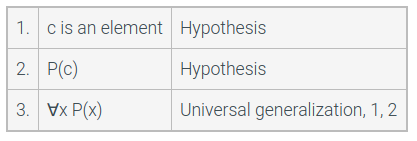
\includegraphics[height=2.8cm]{lecture19-fig2a.png}
     \item[(b)]   True or False? \\
      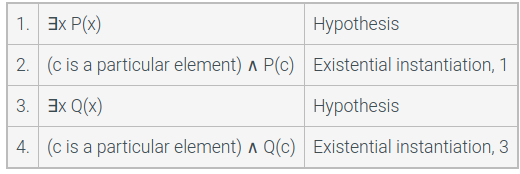
\includegraphics[height=3cm]{lecture19-fig2b.png}
    \end{itemize}
 
 \end{frame}
 
 \begin{frame}[plain]{}

    \begin{itemize}
     \item[(c)]  True or False? \\
      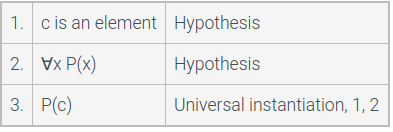
\includegraphics[height=2.8cm]{lecture19-fig2c.png}\ 
    \item[(d)]  True or False? \\
     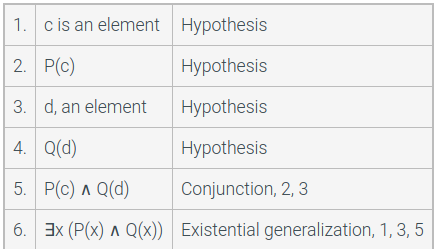
\includegraphics[height=4.5cm]{lecture19-fig2d.png}\ 
    \end{itemize}
 
 \end{frame}
 


\begin{frame}[plain]{}

  {\bf Example 19.4}  Show that the premises 
   "A student in this class has not read the book," and 
   "Everyone in this class passed the first exam" imply the conclusion 
   "Someone who passed the first exam has not read the book."
   \medskip
    \pause
    
    Let $C(x)$ be ``$x$ is in this class," $B(x)$ be ``$x$ has read the book,"
     and $P(x)$ be ``$x$ passed the first exam."\\
     \smallskip
     
    The premises are \Blue{$\exists x (C(x)\wedge \lnot B(x))$} and
    \Blue{$\forall x (C(x)\rightarrow P(x))$}. The conclusion is 
    \Blue{$\exists x (P(x)\wedge \lnot B(x))$}.
     
   \begin{center}
      \begin{tabular}{ll}
        {\bf Step}   & {\bf Reasoning} \\ \pause 
        (1) $\exists x (C(x)\wedge \lnot B(x))$ & Premise \\ \pause
        (2) $C(a)\wedge \lnot B(a)$  & Existential instantiation from (1)\\ \pause 
        (3)  $C(a)$ & Simplification from (2)\\ \pause 
        (4) $\forall x (C(x)\rightarrow P(x))$  & Premise\\ \pause 
        (5) $C(a)\rightarrow P(a)$ & Universal instantiation from (4)\\ \pause
        (6) $P(a)$  & Modus ponens from (3) and (5) \\ \pause
        (7) $\lnot B(a)$  & Simplification from (2) \\ \pause
        (8) $P(a)\wedge \lnot B(a)$ & Conjunction from (6) and (7) \\ \pause
        (9) $\exists x (P(x)\wedge \lnot B(x))$ & Existential generalization from (8)
     \end{tabular}
     \end{center}
  
\end{frame}


\begin{frame}[plain]{}

 {\bf Practice 19.5}. Consider the argument
 \begin{quote}
 "There is a self-driving car that has been involved in a fatal accident.
 All self-driving cars are designed to prioritize passenger safety.
 Therefore, there is a self-driving car designed to prioritize passenger safety that has been involved in a fatal accident.
\end{quote}
Determine whether the argument is valid.
 Justify your answer by
   explaining which rules of inference are used for each step or by
   finding a counterexample.

\vspace{1.5in}
  
\end{frame}


\iffalse %%%%%%%%%%%%
\begin{frame}[plain]{}

\textcolor{blue}{Solution}. 
Let \(\text{SDC}(x)\) mean "x is a self-driving car," \(\text{FA}(x)\) mean "x has been involved in a fatal accident," and \(\text{PS}(x)\) mean "x is designed to prioritize passenger safety." Then, the premises are 
\Blue{
$
\exists x (\text{SDC}(x) \land \text{FA}(x)) \quad \text{and} \quad \forall x (\text{SDC}(x) \rightarrow \text{PS}(x)).
$
}
The conclusion is
\Blue{
$
\exists x (\text{PS}(x) \land \text{FA}(x)).
$
}

\[
\begin{array}{lll}
1. & \exists x (\text{SDC}(x) \land \text{FA}(x)) & \text{Premise} \\
2. & \forall x (\text{SDC}(x) \rightarrow \text{PS}(x)) & \text{Premise} \\
3. & \text{Let } a \text{ be such that } \text{SDC}(a) \land \text{FA}(a) & \text{Existential Instantiation (EI) from 1} \\
4. & \text{SDC}(a) \land \text{FA}(a) & \text{By definition of EI} \\
5. & \text{SDC}(a) & \text{Simplification from 4} \\
6. & \text{FA}(a) & \text{Simplification from 4} \\
7. & \text{SDC}(a) \rightarrow \text{PS}(a) & \text{Universal Instantiation (UI) from 2} \\
8. & \text{PS}(a) & \text{Modus Ponens from 5 and 7} \\
9. & \text{PS}(a) \land \text{FA}(a) & \text{Conjunction from 6 and 8} \\
10. & \exists x (\text{PS}(x) \land \text{FA}(x)) & \text{Existential Generalization (EG) from 9} \\
\end{array}
\]

\end{frame}
\fi%%%%%%%%%%%%%%%

\begin{frame}[plain]{}

{\bf Activity 19.6} 
Consider the following argument based on Asimov's Three Laws of Robotics:
\begin{quote}
1. ``All robots are programmed to prioritize preventing harm to humans above all else.'' \\
2. ``All robots are programmed to obey human orders unless those orders conflict with preventing harm to humans.'' \\
3. ``All robots are programmed to protect their own existence only when it does not conflict with preventing harm to humans or obeying human orders.'' \\
4. ``A robot has been ordered to save a child from a collapsing building on the other side of the street.'' \\
5. ``Therefore, there is a robot that will risk its own destruction to save the child.''
\end{quote}

Formalize this argument in predicate logic and determine its validity by providing a step-by-step proof sequence.

\end{frame}



\end{document}

%%%%%%%%%%%%%%%%%%%%%%%%%%%%%%%%%%%%%%%%%%%
%%%%%%%%%%%%%%%%%%%%%%%%%%%%%%%%%%%%%%%%%%%

\begin{frame}[plain]{}

 {\bf Activity 19.5}. Consider the argument

 \begin{quote}
    “Ahmad is a student in this class who owns a yellow Lamborghini.
    Everyone who owns a yellow Lamborghini has gotten 
      at least one speeding ticket. 
      Therefore, someone in this class has gotten a speeding ticket.” 
    \end{quote}
 Determine whether the argument is valid.
 Justify your answer by
   explaining which rules of inference are used for each step or by
   finding a counterexample.
  %Rosen, Section 1.6, p79, #14
  %\vspace{1in}
  
  
\end{frame}


\begin{frame}[plain]{Universal Modus Ponens}

In Example 19.1, we used both {\bf universal instantiation}, a rule of inference for quantified statements, 
and {\bf modus ponens}, a rule of inference for propositional logic.
We will often need to use this combination of rules of inference,   called \Blue{Universal Modus Ponens}:

\begin{center}
   \includegraphics[height=2cm]{lecture19-fig4.png}
\end{center}
\pause 

{\bf Example 19.5.}
Rewrite the following argument using quantifiers, variables,
and predicate symbols. Is this argument valid? Why?\\
%submaterial

   \ \ \ \ \  ``If an integer is even, then its square is even."\\
   \ \ \ \ \  ``$k$ is a particular integer that is even." \\
   \ \ \ \ \ Therefore, \\
   \ \ \ \ \ "$k^2$ is even." 

\end{frame}

\begin{frame}[plain]{}

{\bf Solution to Example 19.5}.  The major premise of this argument can be rewritten as\\
  \begin{center}
    $\forall x$ if $x$ is an even integer, then $x^2$ is even.
  \end{center}
  
Let $E(x)$ be ``$x$ is an even integer," $S(x)$ be ``$x^2$ is even,”
 and $k$ stand for a particular integer that is even.\\
 \smallskip
 
 Then the argument has the following form:
 \medskip
 
    \ \ \ \ \  $\forall x (E(x)\rightarrow S(x))$\\
   \ \ \ \ \  $E(k)$ for a particular $k$. \\
   \ \ \ \ \ Therefore, \\
   \ \ \ \ \ $S(k)$ \\
   
   \medskip
   
   This argument has the form of universal modus ponens
and is therefore valid.

\end{frame}

\begin{frame}[plain]{Universal Modus Tollens}

  Another useful combination of a rule of inference from propositional logic and a rule of
   inference for quantified statements is 
   \Blue{Universal Modus Tollens}. 
   Universal modus tollens combines universal instantiation and
   modus tollens and can be expressed in the following way:
   \begin{center}
   \includegraphics[height=2cm]{lecture19-fig5.png}
\end{center}
 
 {\bf Example 19.6.} 
  Rewrite the following argument using quantifiers, variables,
and predicate symbols. Write the major premise in
conditional form. Is this argument valid? Why? 
 
 \medskip
 
   \ \ \ \ \  ``All human beings are mortal."\\
   \ \ \ \ \  ``AI is not mortal." \\
   \ \ \ \ \ Therefore, \\
   \ \ \ \ \ "AI is not human." 
   
  \vspace{2in}
  
\end{frame}





%%%%%%%%%%%%%%%%%%%%%%%%%%%
 \item  {\small  Is the given argument valid?
    \begin{center}
      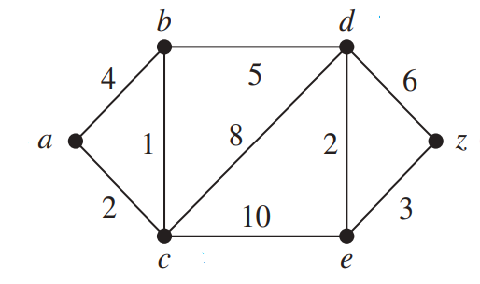
\includegraphics[height=1.8 cm]{../Lecture_F16/lecture7-fig1.png}
    \end{center}
    }
  \item {\small The following whimsical argument was written by Lewis Carroll (author of
 ' Alice's Adventures in Wonderland') and appeared in his 1896 book Symbolic Logic:
 \begin{quote}
  ``No ducks waltz. No officers ever decline to waltz. All my poultry are ducks. Therefore, 
     my poultry are not officers.'' 
 \end{quote}
  Determine whether the argument is valid.
  